% SOURCE_AUTHORITY: sga5_fr_workpass.tex, lines 14277--14318 (LF-normalized unit).
% SOURCE_SHA256: 791F4EFFC5E02832D5D77ED03518C8156D6F07E4C8238B03545DB93D883FBB28
\subsubsection*{n\textsuperscript{o} 2. Morfismo de Frobenius relativo}

Seja $S$ um pré-esquema de característica $p$; todos os $S$-pré-esquemas são também de característica $p$. Se $X$ é um $S$-pré-esquema, vê-se (cf. o diagrama) que $\fr_X$ se fatora através da projeção
\[
\pi_{X/S}:X\times_S(S,\fr_S)\longrightarrow X,
\]
onde $(S,\fr_S)$ denota $S$ considerado como $S$-pré-esquema por meio do morfismo $\fr_S$. Denotaremos o produto fibrado $X\times_S(S,\fr_S)$ por $X^{(p/S)}$, ou mesmo por $X^{(p)}$ se não houver confusão; o único $S$-morfismo de $X$ em $X^{(p/S)}$ que, composto com $\pi_{X/S}$, dá $\fr_X$ denota-se por $\Fr_{X/S}$; obtém-se assim um diagrama comutativo no qual o quadrado é cartesiano:
\[
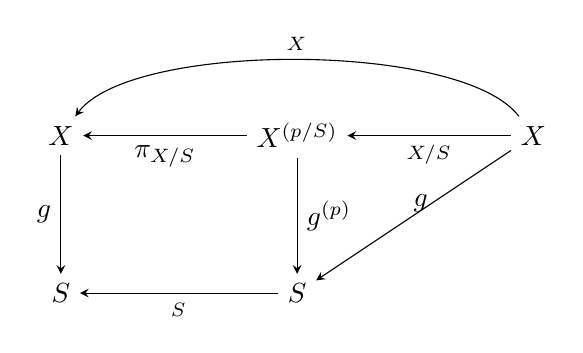
\begin{tikzpicture}[baseline=(current bounding box.center),>=stealth]
\node (XL) at (0,2.0) {$X$};
\node (XM) at (3.0,2.0) {$X^{(p/S)}$};
\node (XR) at (6.0,2.0) {$X$};
\node (SL) at (0,0) {$S$};
\node (SM) at (3.0,0) {$S$};
\draw[->] (XM) -- node[below] {$\pi_{X/S}$} (XL);
\draw[->] (XR) -- node[below] {$\Fr_{X/S}$} (XM);
\draw[->] (XR) .. controls (5.1,3.2) and (0.9,3.2) .. node[above] {$\fr_X$} (XL);
\draw[->] (XL) -- node[left] {$g$} (SL);
\draw[->] (XM) -- node[right] {$g^{(p)}$} (SM);
\draw[->] (XR) -- node[pos=.55,above right] {$g$} (SM);
\draw[->] (SM) -- node[below] {$\fr_S$} (SL);
\end{tikzpicture}
\]

É claro que $X^{(p/S)}$ depende funtorialmente do $S$-pré-esquema $X$; o funtor
\[
p_S:X\longmapsto X^{(p/S)}
\]
é simplesmente a mudança de base mediante o morfismo $\fr_S:S\to S$. Como toda mudança de base, comuta com os limites projetivos e as somas, e conserva propriedades tais como: de tipo finito, separado, afim, projetivo, plano, étale etc. A comutação com os limites projetivos mostra que, se $X$ estiver munido de uma estrutura algébrica, por exemplo de grupo, álgebra etc., $X^{(p/S)}$ ficará naturalmente munido de uma estrutura algébrica da mesma espécie.

Utilizando a funtorialidade de $\fr_X$ em relação a $X$, vê-se que o morfismo $\Fr_{X/S}$ depende funtorialmente do $S$-pré-esquema $X$, de modo que se definiu um morfismo funtorial.
\[
\Fr_{X/S}:\id_{(\Sch)/S}\longrightarrow p_S.
\]

\begin{statement}{Definição 3}
Sejam $S$ um pré-esquema de característica $p$ e $X$ um $S$-pré-esquema. Diz-se que o $S$-morfismo
\[
\Fr_{X/S}:X\longrightarrow X^{(p/S)}
\]
é o morfismo de Frobenius de $X$ relativamente a $S$.
\end{statement}
